\section{LTI}
\label{tag:LTI}
ここではLTIについて述べさせてもらう
LTI(Learning Tools IterOperability)とは、IMS Global Learning Consortium(以下、IMTと呼ぶ)が、異なるプラットフォーム間(異なるLMS上)における学習支援ツールの相互運用を可能とする技術に関する企画を策定し、標準化した規格のことである。LTIに準拠することの具体的なイメージとして、次のようなケースを想定することができる。先代の研究によりできたNSFをツール・プロバイダとし、異なるLMSから利用するケース。
これにより、LTIに準拠することでMoodle、やCanvasなどの異なるLMS間でNSFとの連携を取ることができた。
本研究ではMoodle、Canvasでの起動を行った。
LTIに置ける用語
Tool Provider(ツール・プロバイダ)\\
Tool Provider(ツール・プロバイダ)とは、外部ツールや外部コンテンツのことであり、本研究ではNSFがツールプロバイダとなる。
Tool Consumer(ツール・コンシューマ)\\
Tool Consumer(ツール・コンシューマ)とは、ツール・プロバイダから提供されたツールを使用するLMSのことである。ツール・コンシューマは例として、Canvas,Moodle,Sakai,blackbordなどがある。本研究ではMoodle、Canvasを使用した。
LTIに置ける利点\\
LTI化することにより、様々なLMSからログインすることなくLMSの学習支援ツールとして利用することができる。また、学習支援ツールを、異なるLMSに合わせた設計で作らずに済むことも利点としてあげられる。これによりツール製作者はツールの再利用および、ツールの共有を可能とすることができる。
LTIの利用方法\\
LMS上でTool Provider(ツール・プロバイダ)を使用するには、各LMS上で外部ツールの設定を変更する必要がある。
例として、moodleでは外部ツール設定より、ツール名、ツールURL、コンシューマキー、秘密鍵の設定をする必要がある。これらの設定を得て、moodleからTool Provider(ツール・プロパイダ)を利用することが可能となる。
\begin{figure}[htbp]
  \begin{center}
    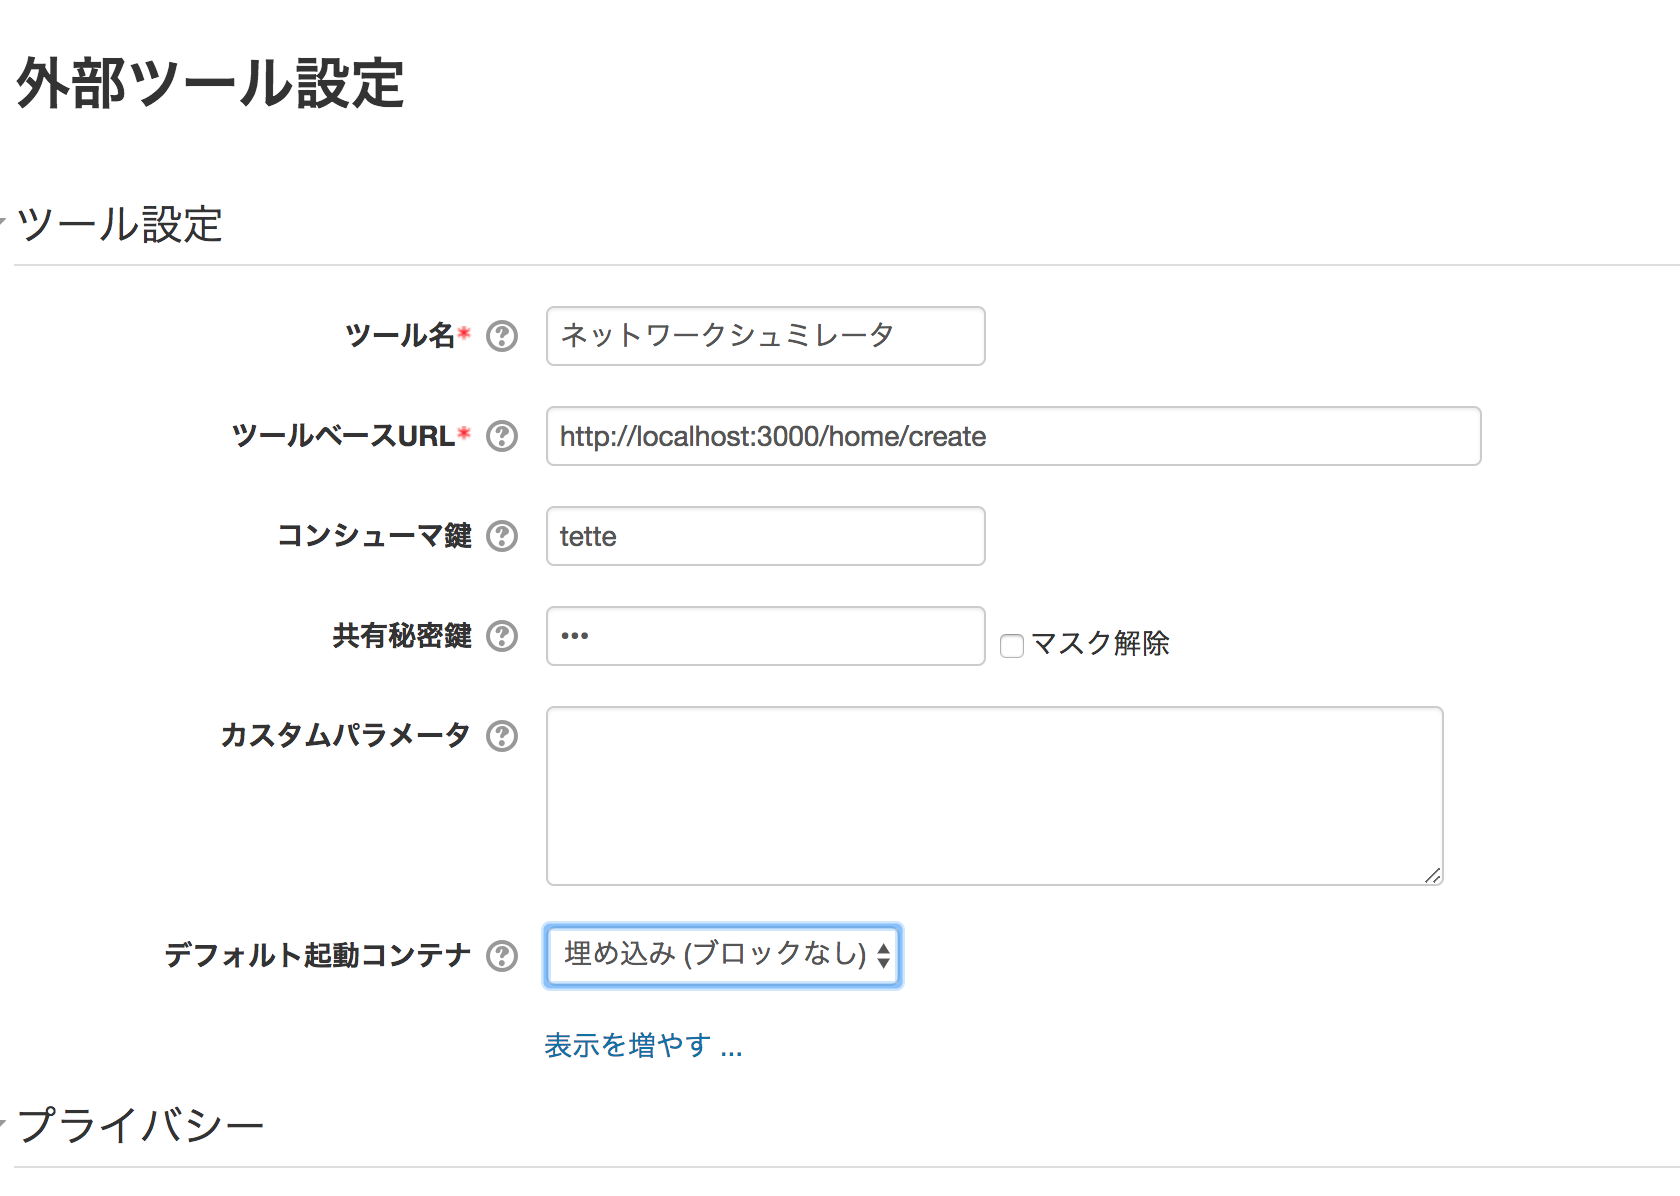
\includegraphics[clip,width=12.0cm,height=8.0cm]{img/moodleSet.png}
    \caption{moodle 外部ツール設定画面}
    \label{fig:moodle config}
  \end{center}
\end{figure}

\begin{figure}[htbp]
  \begin{center}
    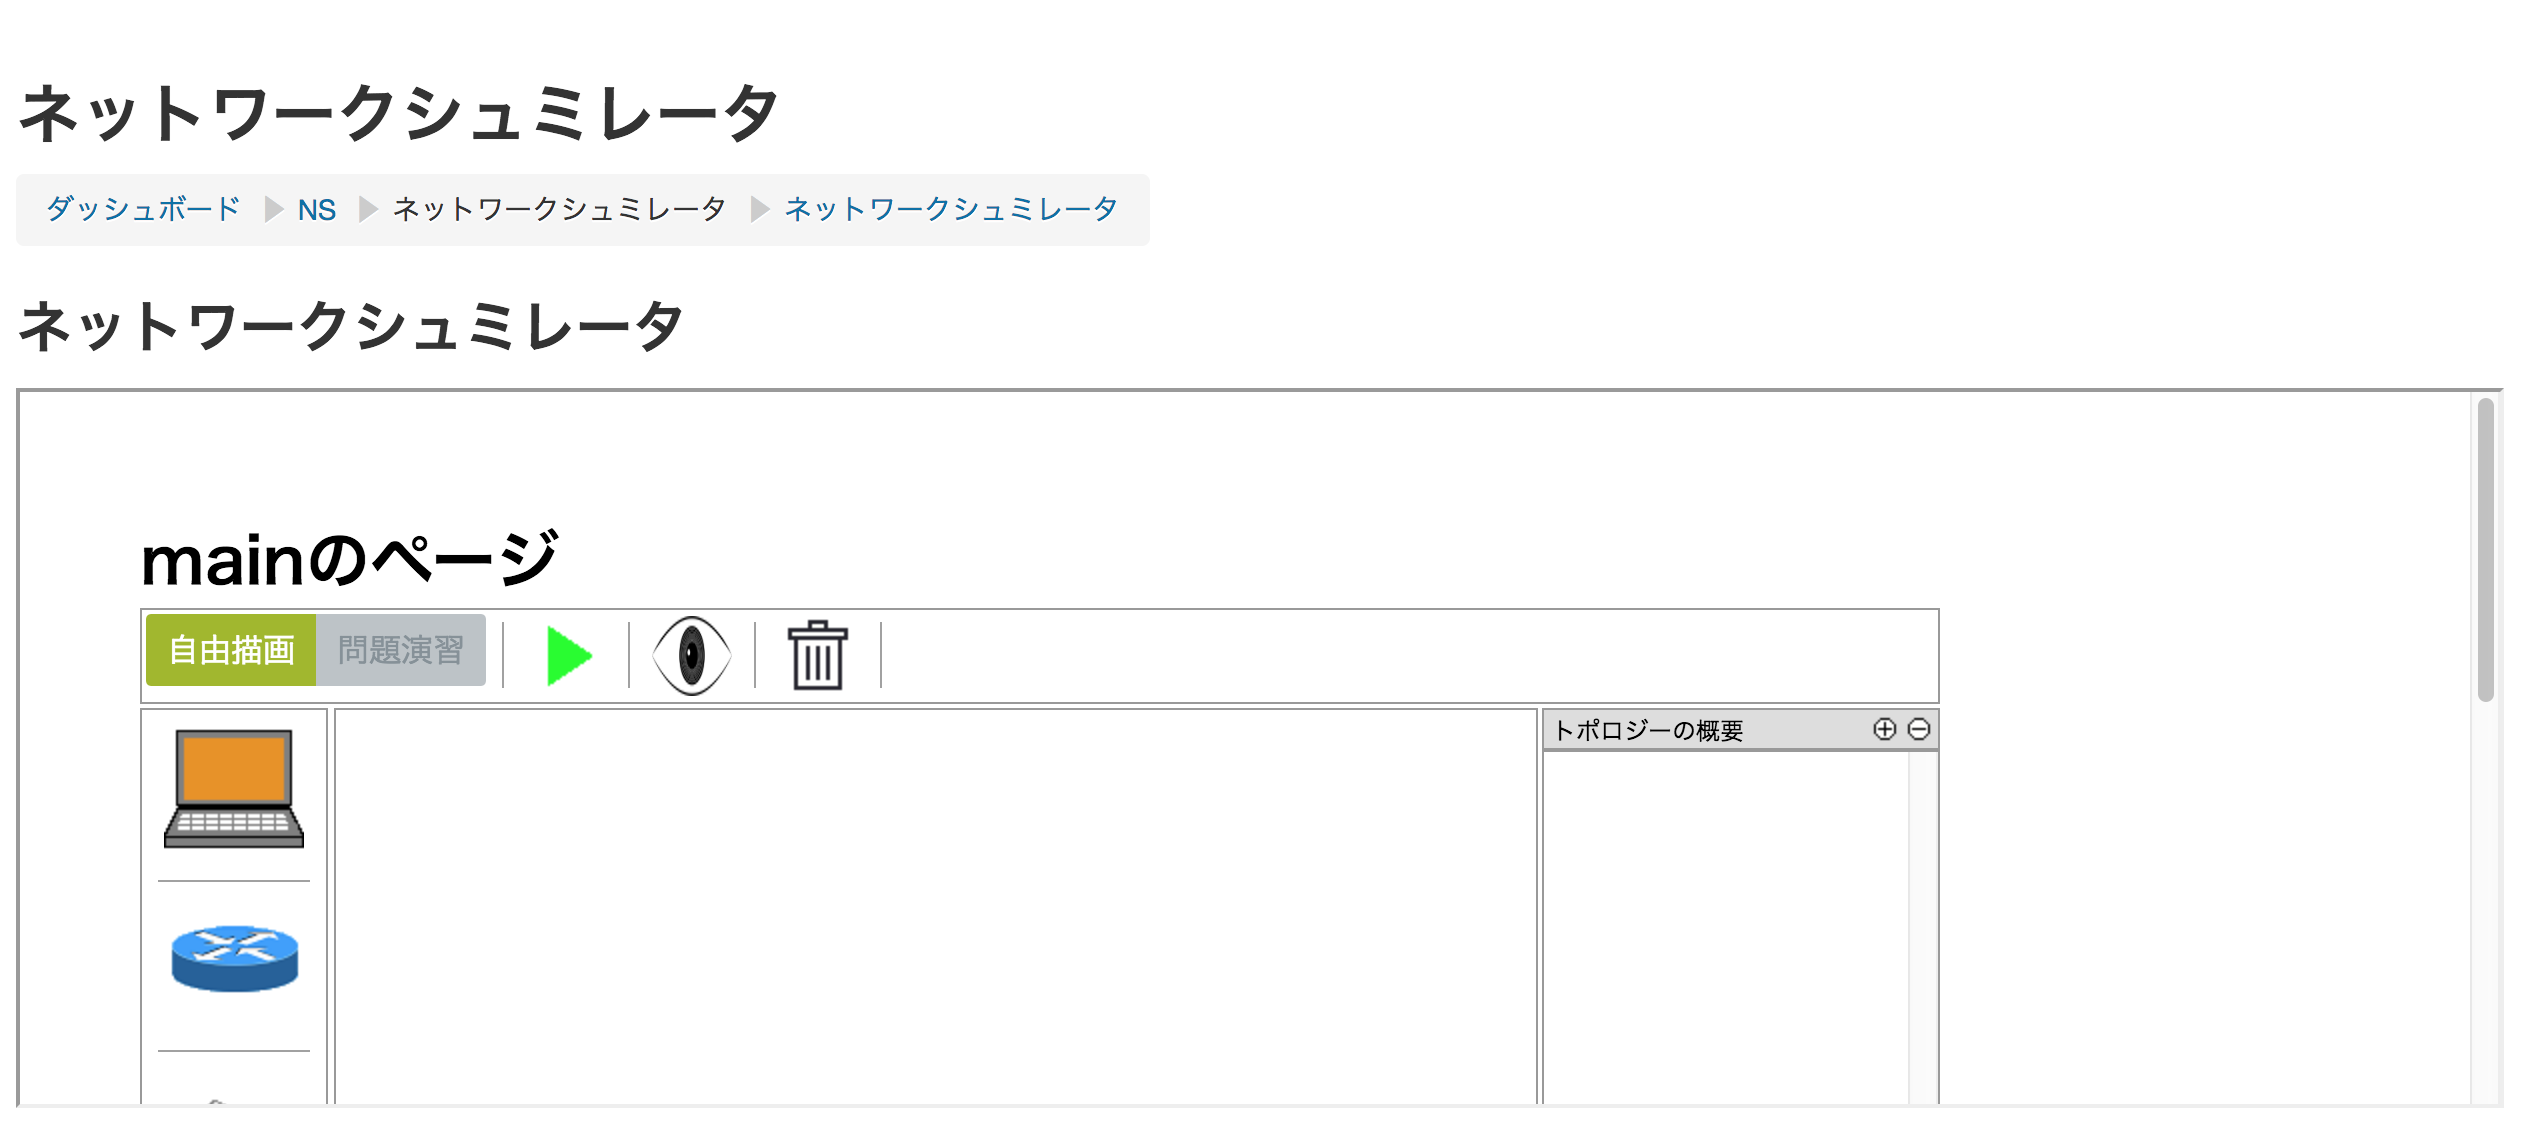
\includegraphics[clip,width=12.0cm,height=8.0cm]{img/LTIstart.png}
    \caption{moodle 外部ツール起動}
    \label{fig:moodle kidou}
  \end{center}
\end{figure}
また、Tool Provider(ツール・プロバイダ),Tool Consumer(ツール・コンシューマ)との間ではOAuth 1.0を使用して認証している\\
OAuth(オーオース)とは、SNSやWebサービス間で[アクセス権限の認可]を行うためのプロトコルである。
これにより、外部ツールへアクセスする際、ユーザIDとパスワードによる認証を行わずに外部ツールへのアクセスを行うことを可能にしている
ここではLTI Tool providerになるための手順について述べさせてもらう
ツールコンシューマから有効なLTI要求をPOSTで送る必要がある。その時必要なパラメータとして、[lti_message_typ]=[basic-lti-launch-request]、[lti_version=[LTI-1p0][oauth_consumer_key]および[resource_link_id]が必須である
[oauth_callback]=[about:blank]、[oauth_consumer_key]=[各自で設定したもの]、[oauth_nonce]=[ランダムに生成された一意の値]、[oauth_signature]=、[oauth_signature_method ],[oauth_timestamp]=,[oauth_version]=[oauth_version]
3,送られてきた情報を元に署名を作成し、送られてきた署名と一致するようならば、ツールプロバイダで行った処理を返す
成績処理について
